	\documentclass[12pt]{article}
\usepackage[utf8]{inputenc}
\usepackage[spanish]{babel}
\usepackage{anysize} 
\usepackage{hyperref}
\usepackage{graphicx}
\usepackage{multirow}
\usepackage{float}
\usepackage{longtable} % para tablas largas
%palabras y su separación 

\hyphenation{res-pecto}
\hyphenation{re-ferente} 
\hyphenation{desa-rrollo}
\hyphenation{mode-lo}

\hyphenation{requeri-mientos}


\usepackage[x11names,table]{xcolor}
\usepackage{color, colortbl}
%\marginsize{2cm}{0cm}{3cm}{1cm} % Controla los márgenes {izquierda}{derecha}{arriba}{abajo}. 
\renewcommand{\figurename}{Figura}
\renewcommand{\refname}{Referencias}
\renewcommand{\contentsname}{Índice}
\renewcommand\tablename{Tabla}
\newcommand{\myparagraph}[1]{\paragraph{#1}\mbox{}\\}

\hypersetup{pdftitle={Archivos PDF},colorlinks=true,%
pdfstartview=Fit,pdfview=Fit,linkcolor=blue}

\begin{document} 
  \newcolumntype{g}{>{\columncolor{gray}}p}
    \begin{tabular}{ |g{3cm}|p{13cm}|} \hline
	\rowcolors{1}{}{gray!20}
	& 
\includegraphics[width=3in]{logo_uach_informatica.png} \\
	&  \\
	& \\
	&  \begin{center}  {\Large {\bf Primer Semestre 2015}} \end{center}	\\
	& \\
	& \\ 
	&  \begin{center}  {\LARGE {\bf Sistema de apoyo al monitoreo curricular de pregrado UACh}} \end{center}	\\
	& \\
	& \\ 
	&  \begin{center}  {\Large {\bf Baldomero Águila Napoli}} \end{center}	\\
	& \\
	& \\ 
	&  \begin{center}  {\Large {\bf \parbox[c]{7cm}{\centering Mauricio Ruiz-Tagle\\	 Patrocinante} }} \end{center}	\\
	& \\
	& \\ 
	& \\

	& \\

	& \begin{center}  {\small {\bf Valdivia, Abril de 2015 }} \end{center} \\ \hline
	\end{tabular}
	\thispagestyle{empty}
	\newpage
	\thispagestyle{empty}
	\tableofcontents
	\newpage
  \setcounter{page}{1}
	
	
	\section{PRESENTACIÓN GENERAL}
		\subsection{Nombre del Proyecto}
			\begin{tabular}{ |c|} \hline
			\\
			 {\large Sistema de apoyo al monitoreo curricular de pregrado UACh}\\
			\\
			 \hline
			
			\end{tabular}
		 
		\subsection{Dominio}
			\begin{tabular}{ |c|} \hline
			\\
			 {\large Informática, Tecnología}\\
			\\
			 \hline
			 \end{tabular}
		\subsection{Área de Aplicación}
			\begin{tabular}{ |c|} \hline
			\\
			 {\large Administración Académica}\\
			\\
			 \hline
			 \end{tabular}
		\subsection{Duración del proyecto}
		
			\begin{tabular}{ |c|c|c|} \hline
			& & \\
			 0 & 8 & {\large Meses }\\
			
			& & \\
			 \hline
			
			\end{tabular}
			\newpage
	\section{RESPONSABLES DEL PROYECTO}
		\subsection{Institución principal del proyecto}
		\begin{large}
			\begin{tabular}{|l|l|}
				\hline
				
					\multicolumn{2}{|p{15cm}|}{ \parbox[t]{15cm}{ {\bf Nombre de la Institución} \\	 Departamento de Aseguramiento de la Calidad e Innovación Curricular (DACIC)}}\\ 
				\hline
				{ \parbox[t]{8cm}{ {\bf Dirección} \\Edificio Vicerrectoría Académica · Campus Isla · Teja · Av. Carlos Ibáñez del Campo}} & { \parbox[t]{8cm}{ {\bf Ciudad} \\	Valdivia}}
		\\ 
		
				\hline
				{ \parbox[t]{8cm}{ {\bf Teléfono} \\	+56 63 2221085}} & { \parbox[t]{8cm}{ {\bf E-mail} \\  dacic@uach.cl}}
		\\ 
		
				\hline

			\end{tabular}
		\end{large}




		\subsection{Patrocinante del proyecto}
		\begin{large}
			\begin{tabular}{|l|l|}
				\hline
				
			{ \parbox[t]{7cm}{ {\bf Nombre Completo} \\	Dr. Jorge Mauricio Ruiz-Tagle Molina}}& { \parbox[t]{7cm}{ {\bf R.U.T.} \\	8.214.713-6}}\\ 
				\hline
				{ \parbox[t]{8cm}{ {\bf Dirección} \\	Campus Miraflores, Valdivia}} & { \parbox[t]{8cm}{ {\bf Ciudad} \\	Valdivia}}
		\\ 
		\hline
							\multicolumn{2}{|p{15cm}|}{ \parbox[t]{15cm}{ {\bf Cargo Actual} \\Académico del instituto de informática}}\\ 
							
				\hline
				{ \parbox[t]{8cm}{ {\bf Teléfono} \\ (56-63) 2221259	}} & { \parbox[t]{8cm}{ {\bf E-mail} \\ mruiztag@uach.cl}}
		\\ 
		
				\hline

			\end{tabular}
		\end{large}
	

		\subsection{Datos del estudiante}
		\begin{large}
			\begin{tabular}{|l|l|}
				\hline
				
			{ \parbox[t]{7cm}{ {\bf Nombre Completo} \\Baldomero Águila Napoli}}& { \parbox[t]{7cm}{ {\bf R.U.T. y Firma} \\	17.536.925-2}}\\ 
				\hline
				{ \parbox[t]{8cm}{ {\bf Dirección} \\	General Lagos 1946}} & { \parbox[t]{8cm}{ {\bf Ciudad} \\	Valdivia}}\\ 

							
				\hline
				
				{ \parbox[t]{8cm}{ {\bf Teléfono} \\ +569-61729928}} & { \parbox[t]{8cm}{ {\bf E-mail} \\ baldomero.napoli@gmail.com}}
		\\ 
		
				\hline

			\end{tabular}
		\end{large}
		\newpage
	\section{RESUMEN DEL PROYECTO}
		
		
		
			"La Universidad Austral de Chile es una institución acreditada que forma profesionales y graduados de pre 
			y postgrado, con un sello caracterizado por la excelencia académica, el compromiso con la libertad y con 
			el medio sociocultural, el respeto por la diversidad, la responsabilidad social, entre otros"\cite{MOD07}. 
			El cumplimiento de estas definiciones establecidas en el \textit{ modelo educacional y enfoque curricular}, requieren, entre otros, de procesos internos de la organización que apoyen la gestión educativa, en particular, de pregrado. Una de las funcionalidades mas importantes en este ámbito, es la gestión de los proyectos curriculares de la carrera. Por esto es de gran importancia el conocer el historial curricular de cada carrera, necesidad que da origen al presente proyecto.
			\\
			
			El objetivo principal del presente proyecto de tesis consiste en diseñar y desarrollar un prototipo de 
			plataforma web que permita gestionar el historial curricular de cada carrera de la Universidad Austral 
			de Chile, el cual permitirá a distintas Unidades de la universidad tener una mejor información curricular 
			de las carreras y así facilitar el trabajo que día a día realizan.
			\\

			
			El sistema web se desarrollará para las dependencias de la Universidad Austral de Chile, es por eso mismo que
			el alumno tesista debe adaptarse a las tecnologías que la universidad utiliza, por esta razón la solución se 
			desarrollará en las siguiente tecnologías: Microsoft Visual Studio 2013, Microsoft SQL Server 2008 
			(solo en ambiente de desarrollo, una vez finalizado el proyecto se migrará a SyBase, el cual es el motor 
			de base de datos que utiliza la universidad), Visual Basic como lenguaje del servidor, JavaScript, css3, HTML5 
			y Tortoise.
			\\

			
			El sistema web beneficiará a los departamentos del área de pregrado de la Universidad en cual están 
			constantemente manipulando información curricular de las carreras, estos departamento son los siguientes: 
			Departamento de Aseguramiento de la Calidad e Innovación Curricular (DACIC), Departamento de Registro 
			Académico Estudiantil y  Departamento de Admisión y Matricula, además beneficiará a la propia escuela, ya que les permitirá contar con
			información histórica curricular.
			\\
			
			Las ventajas de contar con una plataforma web que almacene datos históricos de las carreras, es disminuir el 
			trabajo que poseen estos departamentos al momento de requerir alguna información curricular.

			
			


\newpage
\section{OBJETIVOS GENERALES Y ESPECÍFICOS}
		\subsection{Objetivo General}
			{\large  Diseñar y construir  un prototipo de una plataforma web que apoye al monitoreo curricular de pregrado 
			UACh.}
		\subsection{Objetivos Específicos}
		\begin{large}
			
			\begin{itemize}
				\item Conocer cómo los departamentos que integran la Dirección de Estudios de Pregrado (DEP) administran
				la información referente a los planes de estudios.
				\item  Definir requerimientos del sistema, describiendo sus funcionalidades y separar en módulos la aplicación.
				\item Diseñar e implementar el módulo necesario que permita gestionar el historial curricular de una carrera en particular.
				\item Diseñar e implementar el módulo necesario que permita gestionar el historial de la escuela de una carrera en particular.
				\item Realizar pruebas de validación de los requisitos y estabilidad del prototipo de plataforma web.
			\end{itemize}
		\end{large}
		\newpage
		
	\section{DESCRIPCIÓN DEL PROYECTO}
	
		\subsection{Introducción}
		
		"Durante la última década, las universidades pertenecientes al Consejo de Rectores de Universidades chilenas (CRUCH) 
		han promovido diversas iniciativas de Innovación Curricular" \cite{INN11}. Es por ello que la Universidad Austral de 
		Chile ya ha empezado con el proceso de innovación curricular para que gradualmente abarque todas sus carreras.
		\\
		
		Uno de los principales problemas relacionados con el proceso de calidad e innovación curricular es que la Universidad 
		Austral de Chile almacena toda la información referente al historial curricular de cada carrera en distintos medios 
		de almacenamiento (incluyendo el papel), distintos  formatos, y en varias unidades de la organización, lo que 
		dificulta la generación de informes que apoyen procesos estratégicos de seguimiento y autoevaluación.
		\\
		
		Este proyecto surge como una iniciativa del Dr. Mauricio Ruiz-Tagle quien observó las falencias que tienen los 
		departamentos ya indicados al momento de gestionar documentos relacionados con la innovación curricular.  
		De acuerdo a lo mencionado anteriormente, se pretende crear una plataforma web, que permita gestionar el historial 
		curricular de cada carrera de la universidad, la cual permitirá a distintas Unidades de la universidad tener una 
		mejor información  de las carreras y así facilitar el trabajo que día a día realizan.
		\\
		
		La información obtenida por esta plataforma servirá de apoyo para la gestión curricular por parte de los distintos departamentos que integran la Dirección de Estudios de Pregrado, ya que se contará con todo lo necesario para gestionar los cambios curriculares de los planes de estudio.
		
		
		
	
		

     	 \newpage
     	 
     	 
    

		\subsection{Nivel actual}
		
		Como ya se ha mencionado anteriormente el presente proyecto pretende aportar a los procesos curriculares de la Universidad Austral de Chile, es por esto mismo que es necesario entender los procesos que realizan los departamentos involucrados.
		\\
		
		En la Figura \ref{Figura1} se puede apreciar como se estructuran los departamentos de Vicerrectoría. A partir de este diagrama se explicarán las principales funciones y procesos de los Departamentos de Estudios de Pregrado, los cuales son: Departamento de Aseguramiento de la Calidad de la Docencia e Innovación Curricular, Departamento de Admisión y Matricula y Departamento de Registro Académico Estudiantil.
		
					\begin{figure}[h]
						\centering
						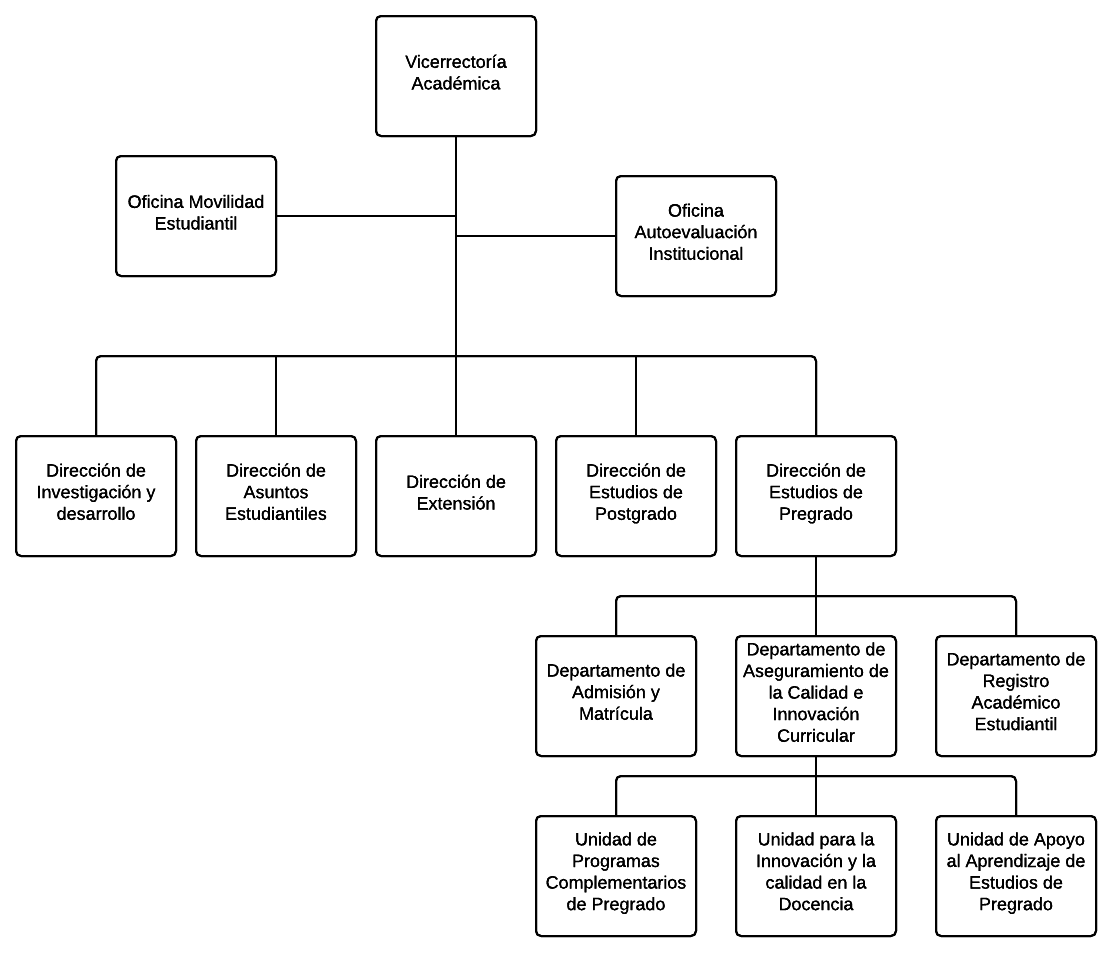
\includegraphics[width=1\textwidth]{Organigrama.png}
						\caption[Organigrama Vicerrectoría y DACIC]{Organigrama Vicerrectoría y DACIC \footnote{}}
						\label{Figura1}
					\end{figure}
					\footnotetext{Elaboración propia.}
		
		\subsubsection{Departamento de Aseguramiento de la Calidad e Innovación Curricular (DACIC)}
		
		
		En este departamento nace la idea de desarrollar un sistema que apoye a los procesos curriculares. Su principal objetivo es ``propender al fortalecimiento de la calidad de los aprendizajes de los estudiantes de la UACh a través del apoyo a las y Docentes en el diseño de situaciones de enseñanza/aprendizaje orientadas a la obtención de resultados efectivos y el asesoramiento a las unidades académicas respectivas en el desarrollo de innovaciones curriculares."\cite{Dac15}
		\\
		
		El departamento está conformado por cuatro Unidades:
		\begin{itemize}
			\item Unidad de Apoyo al Desarrollo de la Docencia de Pregrado
			\item Unidad de Apoyo al Desarrollo y la Innovación Curricular en Pregrado
			\item Unidad de Apoyo al Aprendizaje del Estudiante de Pregrado 	
			\item  Unidad de Programas Complementarios
		\end{itemize}
		
		Sin embargo el proyecto beneficiará directamente  a la Unidad de Apoyo al Desarrollo y la Innovación Curricular en Pregrado, por lo que se dará mas detalles de esta Unidad a continuación.
		
		
		\myparagraph{Apoyo al Desarrollo y la Innovación Curricular en Pregrado}
		
		Unidad encargada de apoyar en el ámbito ``técnico-curricular a las escuelas de Pregrado en sus proyectos de innovación curricular, tanto en carreras profesionales como técnicas, en el contexto del Modelo Educativo y Enfoque Curricular de la Universidad."\cite{Dac15}
		\subsubsection{Departamento de Admisión y Matrícula}
		
			Como su nombre lo indica, este departamento esta presente cuando el alumno ingresa a la Universidad Austral de Chile, en cualquiera de las siguientes modalidades:
			\begin{itemize}
				\item Sistema regular, común a toda la Educación Superior adscrita al Consejo de Rectores de las Universidades Chilenas.
				\item Sistema de Ingreso Especial, propio de la Universidad.
			\end{itemize}
			
			\myparagraph{Servicios estudiantiles} 
			
			\begin{itemize}
				\item 	`` El Departamento de Admisión y Matrícula es la Unidad encargada de otorgar las certificaciones de Alumno Regular a todos los estudiantes de la Universidad, que cumplan con los requisitos para la de emisión de dichos documentos."\cite{Dep15}
				\item Gestiona  la construcción y entrega de las Credenciales Universitarias.
			\end{itemize}
		
			
			
			
		\subsubsection{Departamento de Registro Académico Estudiantil}
	
			Este departamento depende directamente de la Dirección de Estudios de Pregrado de la Vicerrectoría Académica, esta a cargo de la Sra. María Cristina Barriga Ramírez. Entre sus funciones se destaca ``el seguimiento académico del estudiante de pregrado, postítulo y postgrado desde su primera matrícula hasta su egreso y posterior titulación y/o graduación y el permanente apoyo a la labor administrativa que realizan Directores de Escuela, Directores de Unidades Académicas y Profesores en general"\cite{Dir15}.
			
	



			
			\myparagraph{Procesos:}
			
			Esta Unidad  controla la información académica - administrativa, prepara y supervisa los siguientes procesos:
			\begin{itemize}
				\item Peticiones de asignaturas que realizan las Escuelas.
				\item Oferta de asignaturas de las Unidades Académicas.
				\item Inscripción de asignaturas de los estudiantes.
				\item Ingreso de las calificaciones por parte de los profesores.
				\item Modificaciones curriculares de los planes de estudios, de acuerdo  a lo aprobado por la Dirección de Estudios de Pregrado.
				
			\end{itemize}
			
			
			Una vez nombrado los diferentes procesos que controla este departamento, se procederá a explicar los dos  principales procesos que están directamente relacionado con el sistema, los cuales son: Creación de nuevas Carreras y  Modificaciones curriculares de los planes de estudios, de acuerdo  a lo aprobado por la Dirección de Estudios de Pregrado.

			\myparagraph{Creación de nuevas Carreras}
			
			En el diagrama de procesos que se muestra en la Figura \ref{Figura2} describe la secuencia básica que se lleva a cabo para la creación de nuevas carreras en la Universidad Austral de Chile.
			\begin{figure}[H]
				\centering
				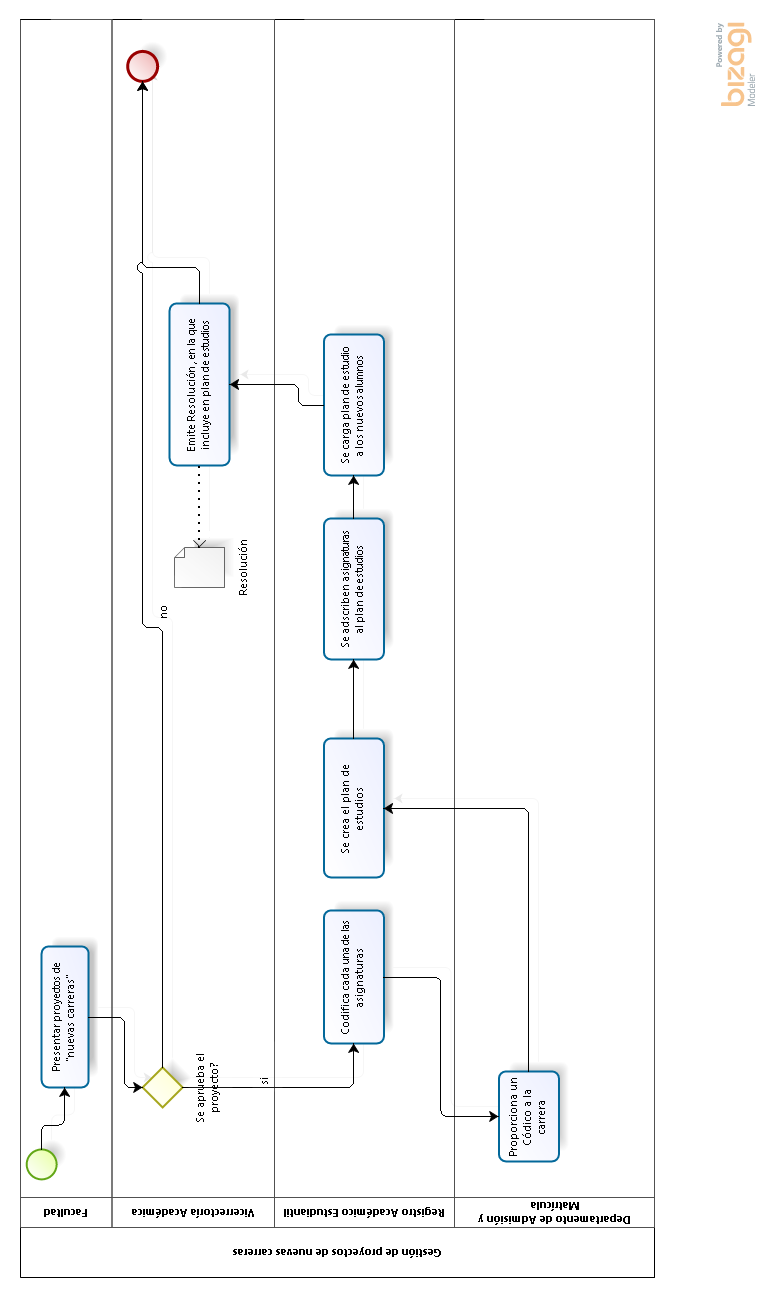
\includegraphics[width=0.9\textwidth]{Procesos_Registro_academico.png}
				\caption[Proceso de presentación de nuevos proyectos]{Proceso de presentación de nuevos proyectos \footnote{}}
				\label{Figura2}
			\end{figure}
			\footnotetext{Elaboración propia.}	
			
			Las fechas para la presentación de nuevos proyectos o innovaciones curriculares, se estipulan en el Decreto de Rectoría  que promulga el Calendario Académico cada año. Para el año 2015 se especifica:
			
			\begin{itemize}
				\item 30 de abril, último día para presentar en la Vicerrectoría Académica, los proyectos de nuevas carreras.
				\item 30 de junio, último día para que las facultades y sedes presenten proyectos de Innovación Curricular de las carreras a la Vicerrectoría Académica.
			\end{itemize}
			
			
			Una vez aprobado una nueva carrera o la innovación curricular por parte de la Vicerrectoría Académica, los pasos administrativos, son los que se indican a continuación:
		
			
			
			
			\begin{enumerate}
				
				
				\item Se codifica cada una de las asignaturas, asociándose a una Unidad Académica especifica. La Unidad Académica es la que le asigna la sigla, en letras y la numeración es un correlativo que se utiliza para la identificación de la asignatura. Ejemplo: CAEV222-14.
				\\
				CAEV = Ciencias Ambientales y evolutivas (Unidad Académica)
				\\
				222   = Numeración asignada para identificarla dentro de la misma unidad.
				\\
				-14    = año de creación (2014)
				
				\item El Departamento de Admisión y Matrícula proporciona  un código a la carrera. Ejemplo 1826, Escuela de Psicología (valdivia).
				
				\item Una vez que las carreras estén creadas y las asignaturas asociadas a una unidad académica, el Departamento de Registro Académico Estudiantil crea el plan de estudios (ver Figura \ref{Figura2}) con la descripción del propio plan:Nombre de bachillerato,Duración, Año de creación,e etc.
				
				\item El proceso final para la creación de una carrera, es cargar  las asignaturas al plan previamente creado, los pasos son los siguientes:
				\begin{enumerate}
					\item Se ingresa una a una las asignaturas previamente creadas.
					\item Se asocia a un semestre en particular.
				\end{enumerate}
			\end{enumerate}
			\newpage
			\myparagraph{Modificaciones Curriculares Mayores y/o Menores}
			
			Tanto la creación de nuevas carreras como todo lo que tiene que ver con modificaciones con respecto al plan de estudio, son proceso que ve el DACIC, específicamente el sub-departamento de Unidad de Apoyo al Desarrollo y la Innovación Curricular en Pregrado, en conjunto con Registro Académico Estudiantil.
			\\
			
			La Figura \ref{Figura2} muestra los procesos administrativos que realiza Registro Académico Estudiantil, a continuación se explicará con mayor detalle.
			El proceso de modificación del plan de estudio comienza con la iniciativa de una escuela, la cual se reúne previamente con Registro Académico Estudiantil, con el objetivo  de identificar quiénes son los afectados por los cambios (número de alumnos, año de ingreso, plan de Estudios, etc.). Una vez concretada esta reunión, la escuela se encuentra en condiciones de formalizar la petición, la cual es enviada a Dirección de Pregrado con la intención de que sea evaluada. En caso de que la petición sea viable, Dirección de Estudios de Pregrado envía una comunicación interna a Registra Académico Estudiantil, informándole que puede efectuar los cambios.
			\\
			
			 Por ultimo Registro Académico Estudiantil realizan una petición de requerimientos al DTI (en caso de que sea necesario, de lo contrario no se efectúa este proceso) para posteriormente aplicar los cambios e informarle a la escuela si Dirección de Pregreado rechazó o aprobó las modificaciones curriculares.
						
			\begin{figure}[H]
				\centering
				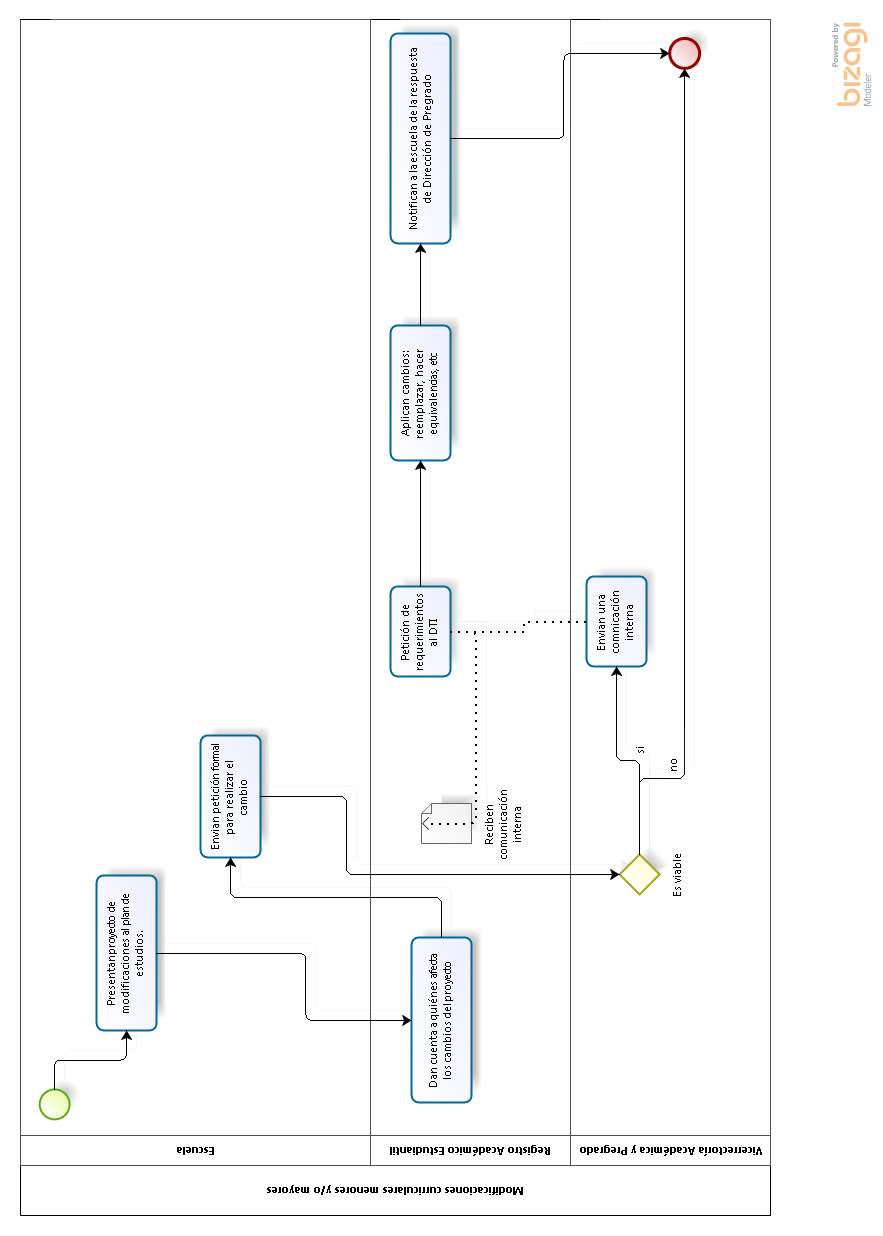
\includegraphics[width=0.9\textwidth]{Procesos_cambios_curriculares.png}
				\caption[Procesos de cambios Curriculares Mayores y/o menores ]{Procesos de cambios Curriculares Mayores y/o menores  \footnote{}}
				\label{Figura2}
			\end{figure}

\footnotetext{Elaboración propia.}				
\newpage


Dado lo anterior, podemos ver que los procesos curriculares no se gestionan con un sistema informático, no existiendo un software encargado  de almacenar y documentar los cambios que afectan a los proyectos curriculares de las carreras.
		\subsection{Motivación}
		Este proyecto cuenta con algunos problemas y/u oportunidades que se presentan a continuación : \\
		\begin{itemize}
		 \item Apoyar la gestión de la documentación virtual de los cambios curriculares que afectan a 
		 las carreras de la Universidad Austral de Chile.
		 \item Aprender nuevas tecnologías.
		 \item Contribuir a mejorar el escaso desarrollo informático para departamentos internos de la Universidad (en este caso la Dirección de Estudios de Pregrado).

		\end{itemize}

 
		\subsection{Impactos}
			El sistema a desarrollar posee los siguientes impactos:
		\begin{itemize}
		\item Se evita la pérdida de tiempo profesional en la búsqueda manual de datos y   documentos. 
		\item  Permite acceso on-line a los documentos desde cualquier lugar de la intranet.
		\item Centralizar toda la información en un solo repositorio de datos.
		\item Mejorar la generación de informes que apoyen procesos estratégicos de seguimiento y autoevaluación.
			
		\end{itemize}
		
		%##########################################################
		% BIBLIOGRAFIA
		
		\renewcommand{\refname}{REFERENCIAS}
		\phantomsection
		\addcontentsline{toc}{section}{REFERENCIAS}
		%----------------------------------------------------------
%----------------------------------------------------------
% BIBLIOGRAFÍA
\begin{spacing}{1.0}
\begin{thebibliography}{99}  

\bibitem [MOD07]{MOD07}
\newblock Universidad Austral de Chile (2007).
\newblock Modelo educacional y enfoque curricular. 

\bibitem [INN11]{INN11}
\newblock Roxana Pey Tumanoff y Sara Chauriye Batarce(2011).
\newblock INNOVACIÓN CURRICULAR EN LAS UNIVERSIDADES DEL CONSEJO DE RECTORES 2000-2010. 


\bibitem [JQu15]{JQu15}
\newblock JQuery
\newblock Disponible en \url{https://jquery.com/}.
\newblock Consultado el 03 de Noviembre de 2015.

\bibitem [eje15]{eje15}
\newblock EjemplosTIW
\newblock Disponible en \url{http://www.lab.inf.uc3m.es/~a0080802/RAI/mvc.html}.
\newblock Consultado el 09 de Noviembre de 2015.

\bibitem [inf15]{inf15}
\newblock Microsoft,Información general sobre ASP.NET
\newblock Disponible en \url{https://msdn.microsoft.com/es-es/library/dd566231.aspx}.
\newblock Consultado el 10 de Noviembre de 2015.


\bibitem [GOM10]{GOM10}
\newblock  Oscar Tinoco Gómez, Pedro Pablo Rosales López \& Julio Salas Bacalla,Criterios de selección de metodologías de desarrollo de software
\newblock 2010
\newblock Disponible en \url{http://www.redalyc.org/articulo.oa?id=81619984009}.
\newblock Consultado el 12 de Noviembre de 2015.


\bibitem [MIC15]{MIC15}
\newblock Microsoft,Usar SQL Server Management Studio
\newblock Disponible en \url{https://msdn.microsoft.com/es-es/library/ms174173%28v=sql.120%29.aspx}.
\newblock Consultado el 10 de Noviembre de 2015.

\bibitem [mic15]{mic15}
\newblock Microsoft SQL Server 2008 Express 
\newblock Disponible en \url{https://www.microsoft.com}.
\newblock Consultado el 05 de Noviembre de 2015.

\bibitem [PAR15]{PAR15}
\newblock Parsleyjs
\newblock Disponible en \url{http://parsleyjs.org/doc/about.html}.
\newblock Consultado el 05 de Noviembre de 2015.

\bibitem [JQu15]{JQu15}
\newblock JQuery
\newblock Disponible en \url{https://jquery.com/}.
\newblock Consultado el 03 de Noviembre de 2015.

\bibitem [gli15]{gli15}
\newblock Blog de Glidea, Qué es un template
\newblock Disponible en \url{http://www.glidea.com.ar/blog/que-es-un-template}.
\newblock Consultado el 04 de Noviembre de 2015.

\bibitem [GIT15]{git15}
\newblock GitHub, github/onokumus
\newblock Disponible en \url{https://github.com/onokumus/Bootstrap-Admin-Template#toc}.
\newblock Consultado el 04 de Noviembre de 2015.

\bibitem [Dac15]{Dac15}
\newblock Departamento de Aseguramiento de la Calidad e Innovación Curricular (DACIC)
\newblock Disponible en \url{http://www.uach.cl/organizacion/direccion-de-pregrado/dacic}.
\newblock Consultado el 07 de Mayo de 2015.

\bibitem [boo15]{boo15}
\newblock Bootstrap
\newblock Disponible en \url{http://getbootstrap.com/about//}.
\newblock Consultado el 04 de Noviembre de 2015.

\bibitem [ALE15]{ALE15}
\newblock AlertifyJS
\newblock Disponible en \url{http://alertifyjs.com/}.
\newblock Consultado el 04 de Noviembre de 2015.

\bibitem [Dep15]{Dep15}
\newblock Departamento de Admisión y Matrícula.
\newblock Disponible en \url{http://www.uach.cl/organizacion/direccion-de-pregrado/admision-y-matricula/departamento-de-admision-y-matricula}.
\newblock Consultado el 05 de Mayo de 2015.


\bibitem [Dir15]{Dir15}
\newblock Dirección de estudios de pregrado.
\newblock Disponible en \url{http://www.uach.cl/organizacion/direccion-de-pregrado/registro-academico}.
\newblock Consultado el 05 de Mayo de 2015.





\end{thebibliography}	
\end{spacing}
		
		
\newpage
\section{RESULTADOS VERIFICABLES RELACIONADOS CON LOS  OBJETIVOS ESPECÍFICOS DEL \\ PROYECTO}

			\begin{tabular}{ |p{15cm}|} \hline
				 \parbox[c]{15cm}{ {\bf Objetivo específico:}\\ \\Conocer cómo los departamentos que integran la 
				 Dirección de Estudios de Pregrado (DEP) administran la información referente a los planes de estudios.\\} 
			\\
			 \hline
				 \parbox[c]{15cm}{ {\bf Descripción del resultado:}\\ 
				 
				 Documento que contenga: \\
				 \begin{itemize}
				  \item Representación de los procesos que afectan el historial curricular.
				  \item Descripción de las funciones de cada departamento de la Dirección de Estudios de Pregrado.
				  \item Modelo entidad Relación
				  \item Estado del arte
				 \end{itemize}
				  Software: \\
				  \begin{itemize}
				   \item Base de datos creada en sql.
						\item Base de datos parcialmente \textit{poblada.}
				  \end{itemize}

			 
				  } 
			 \\ \hline			 
			 \end{tabular}	
			 \\ \\  \\ 
			 
			\begin{tabular}{ |p{15cm}|} \hline
				 \parbox[c]{15cm}{ {\bf Objetivo específico:}\\ \\ Definir requerimientos del sistema, describiendo 
				 sus funcionalidades y separar en módulos la aplicación.\\} 
			\\
			 \hline
				 \parbox[c]{15cm}{ {\bf Descripción del resultado:}\\ 
				 
			Documento que contenga: \\
				 \begin{itemize}
				  \item Especificación  de requisitos funcionales y no funcionales del software.
				  \item Identificación los módulos del software.
				  \item Ciclo de vida del proyecto.
				
				 \end{itemize}
			
				 
				 
				 } 
			 \\ \hline			 
			 \end{tabular}	
			 \\ \\  \\ 
			 
			 \begin{tabular}{ |p{15cm}|} \hline
				 \parbox[c]{15cm}{ {\bf Objetivo específico:}\\ \\Diseñar e implementar el módulo necesario que permita gestionar el historial curricular de una carrera en particular.\\} 
			\\
			 \hline
				 \parbox[c]{15cm}{ {\bf Descripción del resultado:}\\ 
				 
			Documento que contenga: \\
				 \begin{itemize}
				  \item Requisitos funcionales y no funcionales del módulo.
				  \item Artefactos UML del módulo: Diagrama de casos de uso, casos de uso, diagramas de secuencia.
				  \item Mockups de la plataforma.
				
				 \end{itemize}
			Software con las siguientes funcionalidades:\\
			      \begin{itemize}
							\item Estructura principal del proyecto.
							\item La base de datos debe almacenar las resoluciones ingresada por un determinado usuario.
			       \item El software debe ser capaz de visualizar el historial académico por carrera.
			       \item reportes estadísticos.
			     
			      \end{itemize}

				 
				 
				 } 
			 \\ \hline			 
			 \end{tabular}	
			 \\ \\  \\ 
			 
			 			\begin{tabular}{ |p{15cm}|} \hline
				 \parbox[c]{15cm}{ {\bf Objetivo específico:}\\ \\ Diseñar e implementar el módulo necesario que 
				 permita gestionar el historial de la escuela de una carrera en particular.\\} 
			\\
			 \hline
				 \parbox[c]{15cm}{ {\bf Descripción del resultado:}\\ 
				Documento que contenga: \\
				 \begin{itemize}
					 \item 	Especificación de requisitos funcionales y no funcionales.
				  \item Artefactos UML del módulo: Diagrama de casos de uso, casos de uso, diagramas de secuencia.
				  \item Mockups de la plataforma.
				
				 \end{itemize}
			Software con las siguientes funcionalidades:\\
			      \begin{itemize}
				\item Administración del historial de una escuela (\textit{CRUD}).
			       \item Administración de usuarios.
			       \
			     
			      \end{itemize}

				 
					} 
			 \\ \hline			 
			 \end{tabular}	
			 \\ \\  \\ 
			 
			\begin{tabular}{ |p{15cm}|} \hline
				 \parbox[c]{15cm}{ {\bf Objetivo específico:}\\ \\  Realizar pruebas de validación de los requisitos y estabilidad del prototipo de
plataforma web.\\} 
			\\
			 \hline
				 \parbox[c]{15cm}{ {\bf Descripción del resultado:}\\ 
				Documento que contenga: \\
				 \begin{itemize}
				  \item Manual del sistema.
				  \item Hacer pruebas con distintas resoluciones.
				
				 \end{itemize}
		

				 
					} 
			 \\ \hline			 
			 \end{tabular}	
			 \\ \\  \\ 
			 

	
	\newpage

\section{DESCRIPCIÓN DE LA METODOLOGÍA}

Para el desarrollo del proyecto  se utilizará un ciclo de vida {\bf iterativo incremental}, en donde se contará con reuniones periódicas con el Profesor Mauricio Ruiz-Tagle  con el fin de validarlos objetivos.
\\

\textbf{Objetivo específico 1:} Conocer cómo los departamentos que integran la Dirección de Estudios de Pregrado (DEP) administran
								la información referente a los planes de estudios.
								\\
								
Para llevar a cabo el objetivo 1 el alumno trabajará en las oficinas del DACIC, con el objetivo  de  entender el contexto actual de problema, una vez que el alumno entienda el contexto en el cual se pretende desarrollar la aplicación, se  debe crear el modelo de dato. Además el alumno deberá leer materiales bibliográficos  referentes a la problemática que aborda el proyecto actual con la intención de entender los procesos internos administrativos de los departamentos involucrados.
\\
					
\textbf{Objetivo específico 2:} Definir requerimientos del sistema, describiendo sus funcionalidades y separar en módulos la aplicación.
\\

Para ello, primero se deben realizar reuniones con el profesor patrocinante con el fin de describir las principales funcionalidades del sistema general. Una vez realizado esto se debe dividir la aplicación en los posibles módulos, que tiene como objetivo   identificar los incrementos del proyecto y así construir la planificación de este mismo.  
\\

\textbf{Objetivo específico 3:} Diseñar e implementar el módulo necesario que permita desplegar el historial curricular de una carrera en particular.
\\


Para ello, primero se tiene que describir la especificación de requerimientos del módulo \textit{historial curricular} de la plataforma a desarrollar, esto con ayuda del patrocinante. Luego, se debe diseñar el módulo  \textit{historial curricular}, lo cual incluye arquitectura software de la plataforma, artefactos UML y una interfaz que de soporte todos los requerimientos del modulo en particular.Para finalizar, se debe implementar el módulo. Se deben concretar reuniones periódicas con el patrocinante  para monitorear el proceso.
\\

\textbf{Objetivo específico 4:} Diseñar e implementar el módulo necesario que permita desplegar el historial de la escuela de una carrera en particular.\\


Para ello, primero se tiene que describir la especificación de requerimientos del módulo encargado de desplegar el historial de una escuela, esto con ayuda del patrocinante. 
Luego, se debe diseñar el módulo, lo cual incluye artefactos UML y complementar el modelo de datos confeccionado en el objetivo específico 1. Posteriormente, se debe implementar el módulo. Para finalizar, se deben realizar pruebas al módulo en cuestión.
\\

\textbf{Objetivo específico 5:}  Realizar pruebas de validación de los requisitos y estabilidad del prototipo de
plataforma web.

Para ello, se procederá a realizar la integración todos los  módulos. Posteriormente se deben crear algunos casos de prueba, para ver el desempeño de la plataforma. Una vez finalizada la etapa de "testeo", se debe documentar la plataforma, además se deben concretar reuniones periódicas con el patrocinante para monitorear el proceso.
				
				
				
\section{EXISTENCIA DE AVANCES RELACIONADAS CON EL PROYECTO}
	No existen avaneces relacionados con el proyecto.
\section{PRODUCTOS E IDENTIFICADORES DE LOGROS}



\begin{center}
	\begin{longtable}{|p{4cm}|p{4cm}|p{3cm}|p{4cm}|}
		\caption{ Indicadores de Logros} \label{grid_mlmmh} \\
		
		\hline \multicolumn{1}{|c|}{\textbf{Objetivos}} & \multicolumn{1}{c|}{\textbf{Actividades}} & \multicolumn{1}{c|}{\textbf{Subproducto}} & \multicolumn{1}{c|}{\textbf{Indicador de logro}} \\ \hline 
		\endfirsthead
		
		\multicolumn{4}{c}%
		{{\bfseries \tablename\ \thetable{} --Continuación de la página anterior}} \\
		\hline \multicolumn{1}{|c|}{\textbf{Objetivos}} &
		\multicolumn{1}{c|}{\textbf{Actividades}} &
		\multicolumn{1}{c|}{\textbf{Subproducto}}&
		\multicolumn{1}{c|}{\textbf{Indicador de logro}} \\ \hline 
		\endhead
		
		\hline \multicolumn{4}{|c|}{{Continua en la siguiente página}} \\ \hline
		\endfoot
		
		\hline \hline
		\endlastfoot

		
			&  Leer y entender la literatura que aborda el problema (modelo educacional UACh, resoluciones, reglamento de Escuela de  Pregrado, entre otros.).& Lista con los documentos que se deben leer en detalle. & Número de documentos a lo menos 6.\\ 		\cline{2-4}
			
			Conocer cómo los departamentos que integran la Dirección de Estudios de Pregrado (DEP) administran
			la información referente a los planes de estudios.
			
			& Realizar estado del arte. &Documento que contenga una descripción de los procesos curriculares relacionadas con la problemática. & Listar todos los departamentos involucrados y los procesos administrativos de cada uno.\\ \cline{2-4}
			& Modelar Base de datos & Modelo Entidad relación y script en sql. & Aprobación del patrocinante \\ \cline{2-4}
			& Escritura  & Documento formal de tesis (Objetivo 1). & Aprobación Patrocinante.\\ 	\hline
			



			& Definir ciclo de vida de desarrollo de software & Documento que describa el ciclo de vida. & Revisión y aprobación del patrocinante.\\ 		\cline{2-4}
			
			 Definir requerimientos del sistema, describiendo sus funcionalidades y separar en módulos la aplicación.
			
			& Describir las funcionalidades del sistema. & Documento con las funcionalidades del sistema. & Aprobación del patrocinante. \\ \cline{2-4}
			& Identificar todos los módulos  & Documento con los módulos del software  & Aprobación del patrocinante \\	\hline
		
		
		
		& Toma de requisitos &Documento de especificación de requisitos. & Revisión y aprobación del patrocinante.\\ 		\cline{2-4}
		
		Diseñar e implementar el módulo necesario que permita gestionar el historial curricular de una carrera en particular.
		
		& Confeccionar artefactos UML & Documento que contenga los artefactos UML: Diagrama de casos de uso, casos de uso, diagramas de secuencia, diagrama de complemento. & Aprobación Patrocinante.\\ 		\cline{2-4}
		
		& Implementación del módulo historial curricular & Versión preliminar del módulo. & Aprobación Patrocinante.\\ 	\cline{2-4}
		& Testeo y validación del módulo estudiantes. &Versión del módulo validada. & Aprobación Patrocinante.\\ 	
		\hline
		
		
		
		
		
		& Toma de requisitos &Documento de especificación de requisitos. & Revisión y aprobación del patrocinante.\\ 		\cline{2-4}

	Diseñar e implementar el módulo necesario que permita gestionar el historial de la escuela de una carrera en particular
		
		& Confeccionar artefactos UML & Documento que contenga los artefactos UML: Diagrama de casos de uso, casos de uso, diagramas de secuencia, diagrama de complemento. & Aprobación Patrocinante.\\ 		\cline{2-4}
		
		& Implementación del módulo historial curricular & Versión preliminar del módulo. & Aprobación Patrocinante.\\ 	\cline{2-4}
		& Testeo y validación del módulo estudiantes. &Versión del módulo validada. & Aprobación Patrocinante.\\ 	
		\hline
		
		
		
	
		
		
		
		& Integración de los módulos.		& Versión de la plataforma integrada. & Aprobación Patrocinante.\\ 		\cline{2-4}
		
		Realizar pruebas de validación de los requisitos y estabilidad del prototipo de plataforma web.
		& Pruebas de validación: Subir resoluciones, ver historial académico, generación de informes, Ver historial de una escuela. & Versión final de la plataforma validada.& Aprobación Patrocinante.\\ \cline{2-4}
		& Documentar plataforma. & Documento que contenga el manual de usuario de la plataforma. & Aprobación Patrocinante.\\ \hline 
		
		
	
		
		
		
	\end{longtable}
\end{center}
\section{DESCRIPCIÓN DEL ROL DE LOS INTEGRANTES DE EQUIPO DE TRABAJO}
	
		\begin{tabular}{|l|c|p{6cm}|} \hline
			
			Nombre & Rol & Tiempo dedicación al Proyecto. (horas semanales)\\ \hline
			Mauricio Ruiz-Tagle & Patrocinante & 1 \\ \hline
		
			Baldomero Águila Napoli & Tesista &20 \\ \hline
			
		\end{tabular}

	\newpage
\section{PLAN DE TRABAJO }

En la Figura \ref{DiagramaGantt} se muestra la carta gantt correspondiente al presente proyecto.
\begin{figure}[h!]
	\centering
	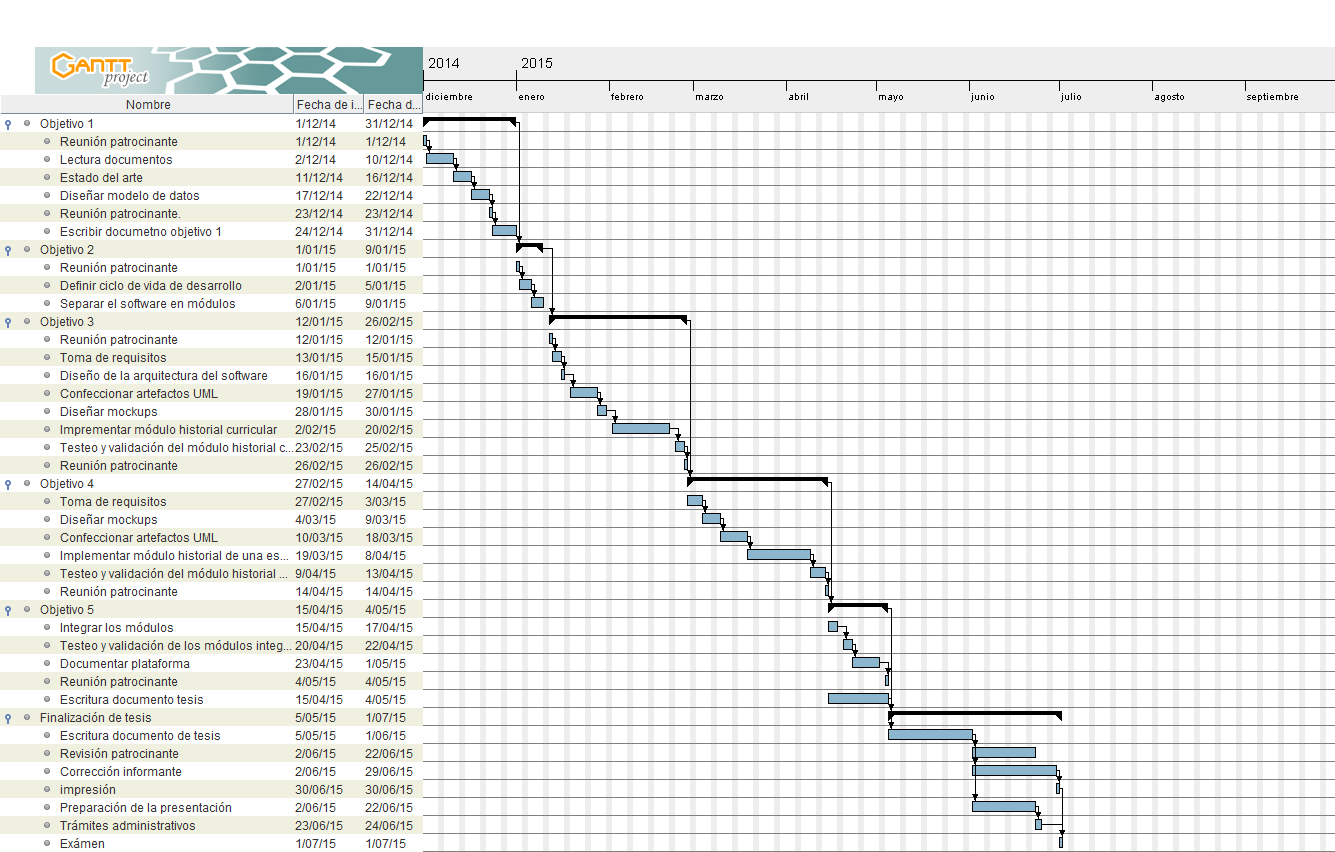
\includegraphics[width=1\textwidth]{carta_gantt.png}
	\caption[Carta Gantt]{Carta Gantt \footnote{}}
	\label{DiagramaGantt}
\end{figure}
\footnotetext{Elaboración propia.}
\section{PRESUPUESTO DE PROYECTO }

	\begin{center}
		
		
		\begin{tabular}{p{1cm}p{2cm}|p{2.1cm}|p{2.1cm}|c|c|}
			\cline{3-4}
			& & \multicolumn{2}{ |c| }{Aportes de terceros} \\ \cline{1-5}
			\rowcolor[gray]{0.6} \multicolumn{1}{ |c| }{ Ítem } & Aporte Ejecutor & Instituto informática & DACIC & Total     \\ \hline
			\multicolumn{1}{ |c| }{ Incentivos y horarios }&\$800.000  & - & - & \$800.000      \\ \hline
			\multicolumn{1}{ |c| }{ Costos de programación  }& \$320.000 & - & - &    \$320.000   \\ \hline
			\multicolumn{1}{ |c| }{ Pasajes y viáticos} & \$256.000  & - & - &  \$256.000      \\ \hline
			\multicolumn{1}{ |c| }{ Equipamiento} & \$350.000 & - & - &    \$350.000    \\ \hline
			\multicolumn{1}{ |c| }{ Materia Fungible }& - & - & - & -      \\ \hline
			\multicolumn{1}{ |c| }{ Difusión} & - & - & - & -      \\ \hline
			\multicolumn{1}{ |c| }{ Gastos Generales }& - &-  &-  &-       \\ \hline
			\rowcolor[gray]{0.6} \multicolumn{1}{ |c| }{ Total} & \$1.726.000 &  &  & \$1.726.000      \\ \hline \hline
			\rowcolor[gray]{0.6} \multicolumn{1}{ |c| }{ Porcentajes }&100\%& 0\% & 0\% &        \\ \hline 
		\end{tabular}
	\end{center}
	
	
	\subsection{Justificación}
	\begin{itemize}
		\item {\bf Incentivos y horarios:} Se considera como incentivos por el proyecto un total de \$100.000 pesos mensuales durante 8 meses, los cuales serán puestos solo por el ejecutor. Esto da un total de \$800.000 pesos.
		
		\item {\bf Costos de programación:}  El alumno diariamente trabaja en la biblioteca Municipal de Osorno, por lo que en este ítem se esta considerando los costos de pasajes y muchas veces colación, lo que da un monto mensual de \$40.000.
		
		
	
		
		\item {\bf Pasajes y viáticos:} Como el alumno se encuentra trabajando en Osorno, y las reuniones se llevan a cabo en Valdivia, el Alumno tesista debe viajar semanalmente a Valdivia, por lo que esta gastando por cada viaje \$8.000, considerando que el proyecto se pretende terminar en 8 meses, el alumno tesista gastará un total de \$256.000
		
		
		\item {\bf Equipamiento:} Notebook con un costo de \$350.000
		
		
	\end{itemize}
	
	
\section{PLAN DE DIFUSIÓN DEL PROYECTO }
	
	\begin{itemize}
		\item Documento de tesis
		\item Examen
	\end{itemize}
	

\end{document}
